%
% domain.tex -- interior point, boundary point
%
% (c) 2019 Prof Dr Andreas Müller, Hochschule Rapperswil
%
\documentclass[tikz,12pt]{standalone}
\usepackage{amsmath}
\usepackage{times}
\usepackage{txfonts}
\usepackage{pgfplots}
\usepackage{csvsimple}
\usetikzlibrary{arrows,intersections,math}
\begin{document}
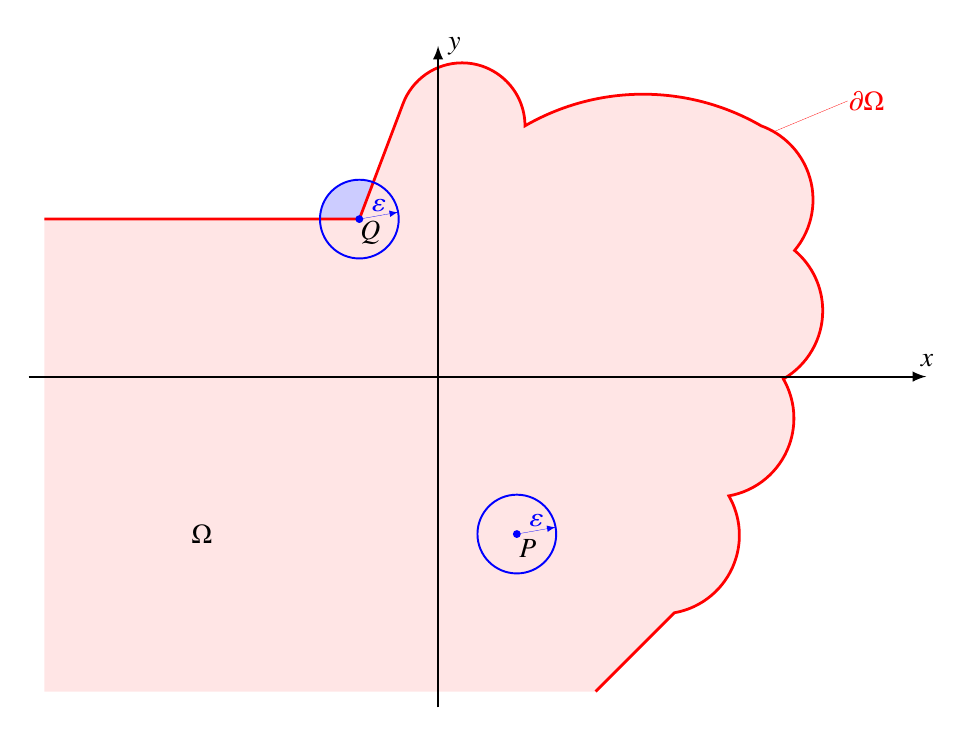
\begin{tikzpicture}[>=latex]

\draw[color=red,line width=0.1pt] (4,3)--(5.2,3.5);

\fill[color=blue!20] (-1,2) circle[radius=0.5];

\fill[color=red!10]
	(-5,2)--(-5,-4)--(2,-4)--(3,-3)
		arc (-80:30:1)
		arc (-80:30:1)
		arc (-60:50:1)
		arc (-40:70:1)
		arc (60:120:3)
		arc (0:160:0.8)
		--(-1,2)
		--cycle;
\draw[color=red,line width=1pt]
	(2,-4)--(3,-3)
		arc (-80:30:1)
		arc (-80:30:1)
		arc (-60:50:1)
		arc (-40:70:1)
		arc (60:120:3)
		arc (0:160:0.8)
		--(-1,2)
		--(-5,2);

\draw[->,line width=0.7pt] (-5.2,0)--(6.2,0) coordinate[label={$x$}];
\draw[->,line width=0.7pt] (0,-4.2)--(0,4.2) coordinate[label={right:$y$}];

\node at ({-1-0.12},{2+0.1}) [below right] {$Q$};
\node at ({1-0.1},{-2+0.05}) [below right] {$P$};

\def\a{10}

\draw[->,color=blue,line width=0.1pt] (-1,2)--({-1+0.5*cos(\a)},{2+0.5*sin(\a)});
\draw[->,color=blue,line width=0.1pt] (1,-2)--({1+0.5*cos(\a)},{-2+0.5*sin(\a)});

\node[color=blue] at ({-1+0.25*cos(\a)},{2+0.25*sin(\a)-0.08}) [above] {$\varepsilon$};
\node[color=blue] at ({1+0.25*cos(\a)},{-2+0.25*sin(\a)-0.08}) [above] {$\varepsilon$};

\fill[color=blue] (-1,2) circle[radius=0.05];
\fill[color=blue] (1,-2) circle[radius=0.05];

\draw[color=blue,line width=0.7pt] (-1,2) circle[radius=0.5];
\draw[color=blue,line width=0.7pt] (1,-2) circle[radius=0.5];

\node at (-3,-2) {$\Omega$};

\node[color=red] at (5.1,3.5) [right] {$\partial\Omega$};

\end{tikzpicture}
\end{document}

